As mentioned in the Methodology section~\ref{sec:methodology}, the first step was to analyse time series the the anemometers and thermocouples averaged in a 30 minute period. In figure~\ref{fig:temp_series} we show the temperature time series for the CSAT3 and the thermocouples, for the whole campaign.

Note: from this time series and according to the criteria for choosing a good nigth to analyse with a smaller averaging period, we selected the nights of the 16th to the 17th, the nights of the 22th to the 23th and the nights from the 23th to the 24th of February (marked in figure~\ref{fig:temp_series} as a yellow shadow). 

\begin{sidewaysfigure}
  \centering
  {
  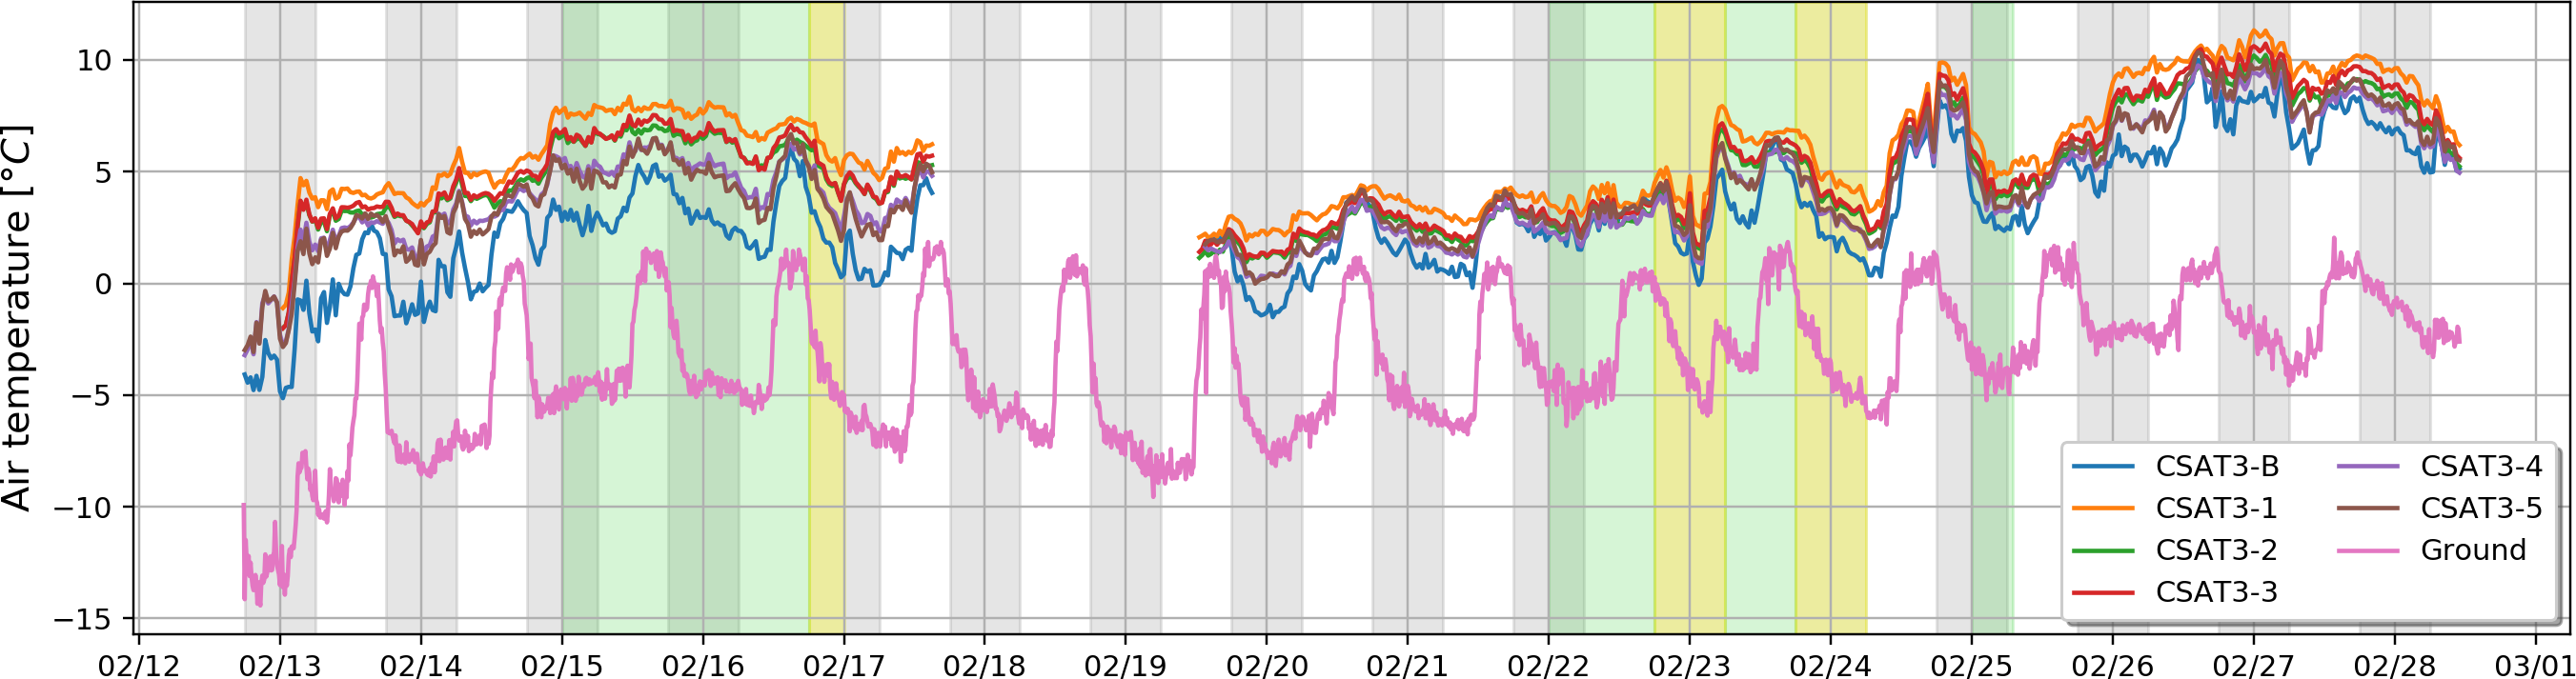
\includegraphics[width=1\textwidth]{fig/chapter_4/T_series_csat.png}\\
   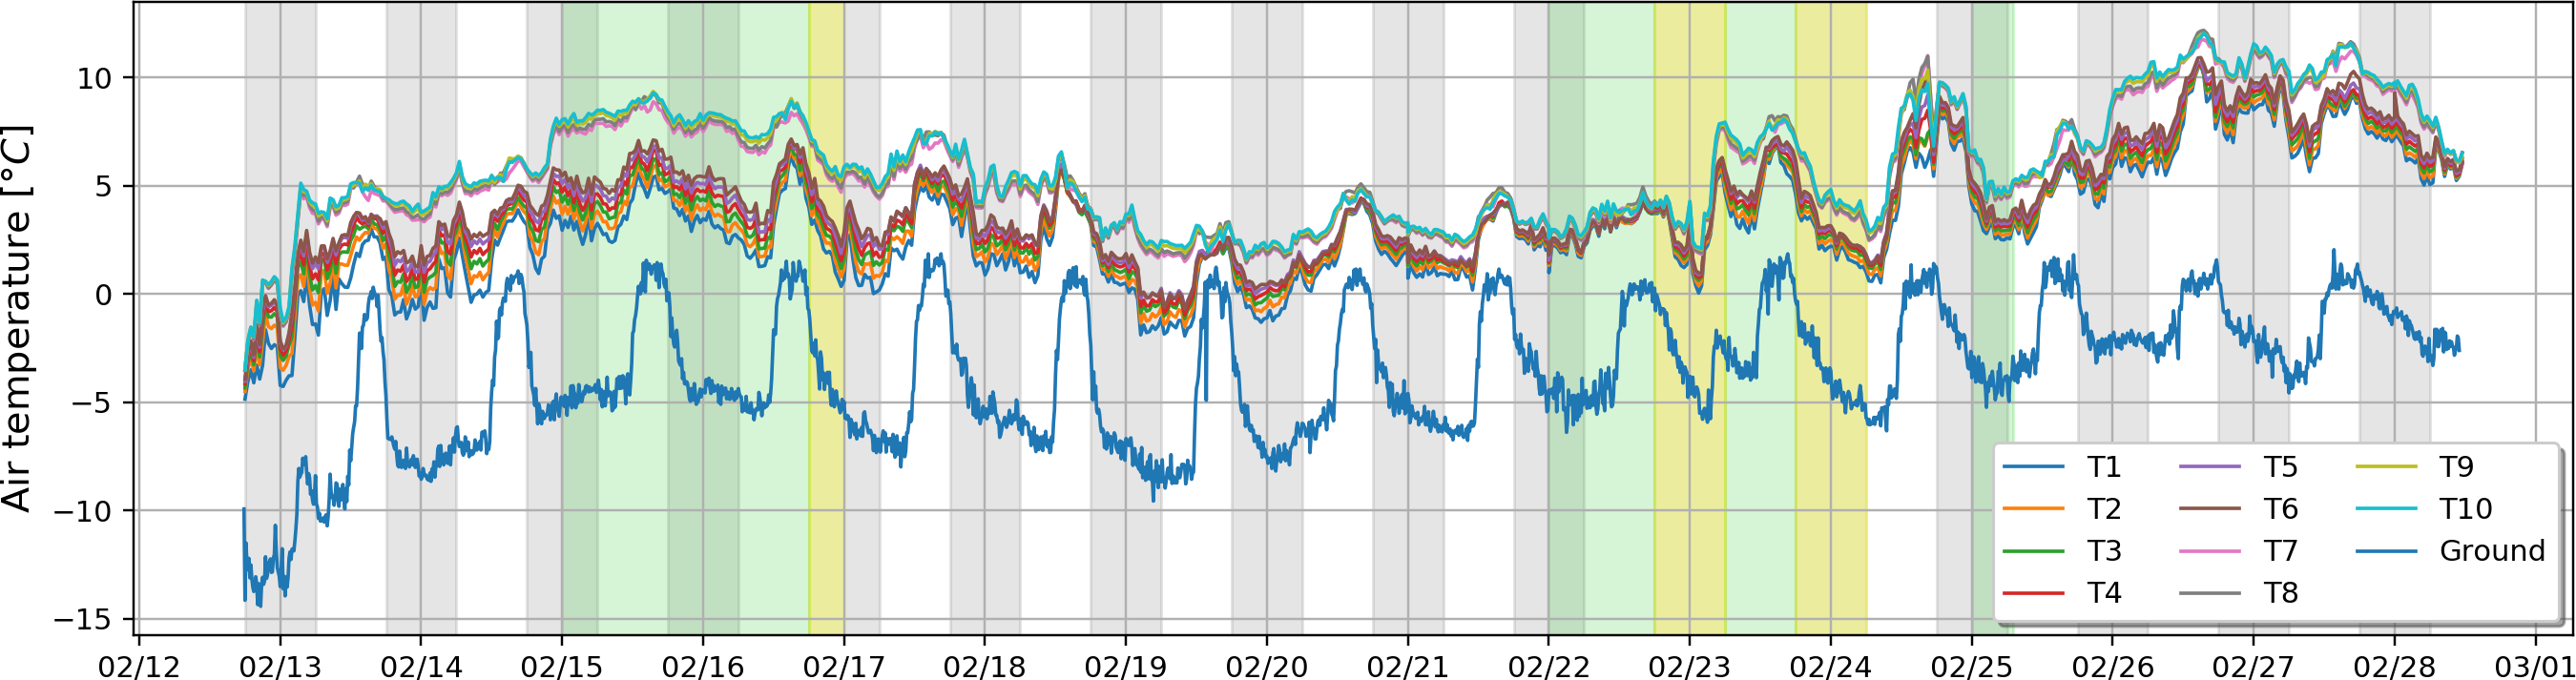
\includegraphics[width=1\textwidth]{fig/chapter_4/T_series_thermocouple.png}
   }
  \caption{}
  \label{fig:temp_series}
\end{sidewaysfigure}

\begin{sidewaysfigure}
  \centering
  {
  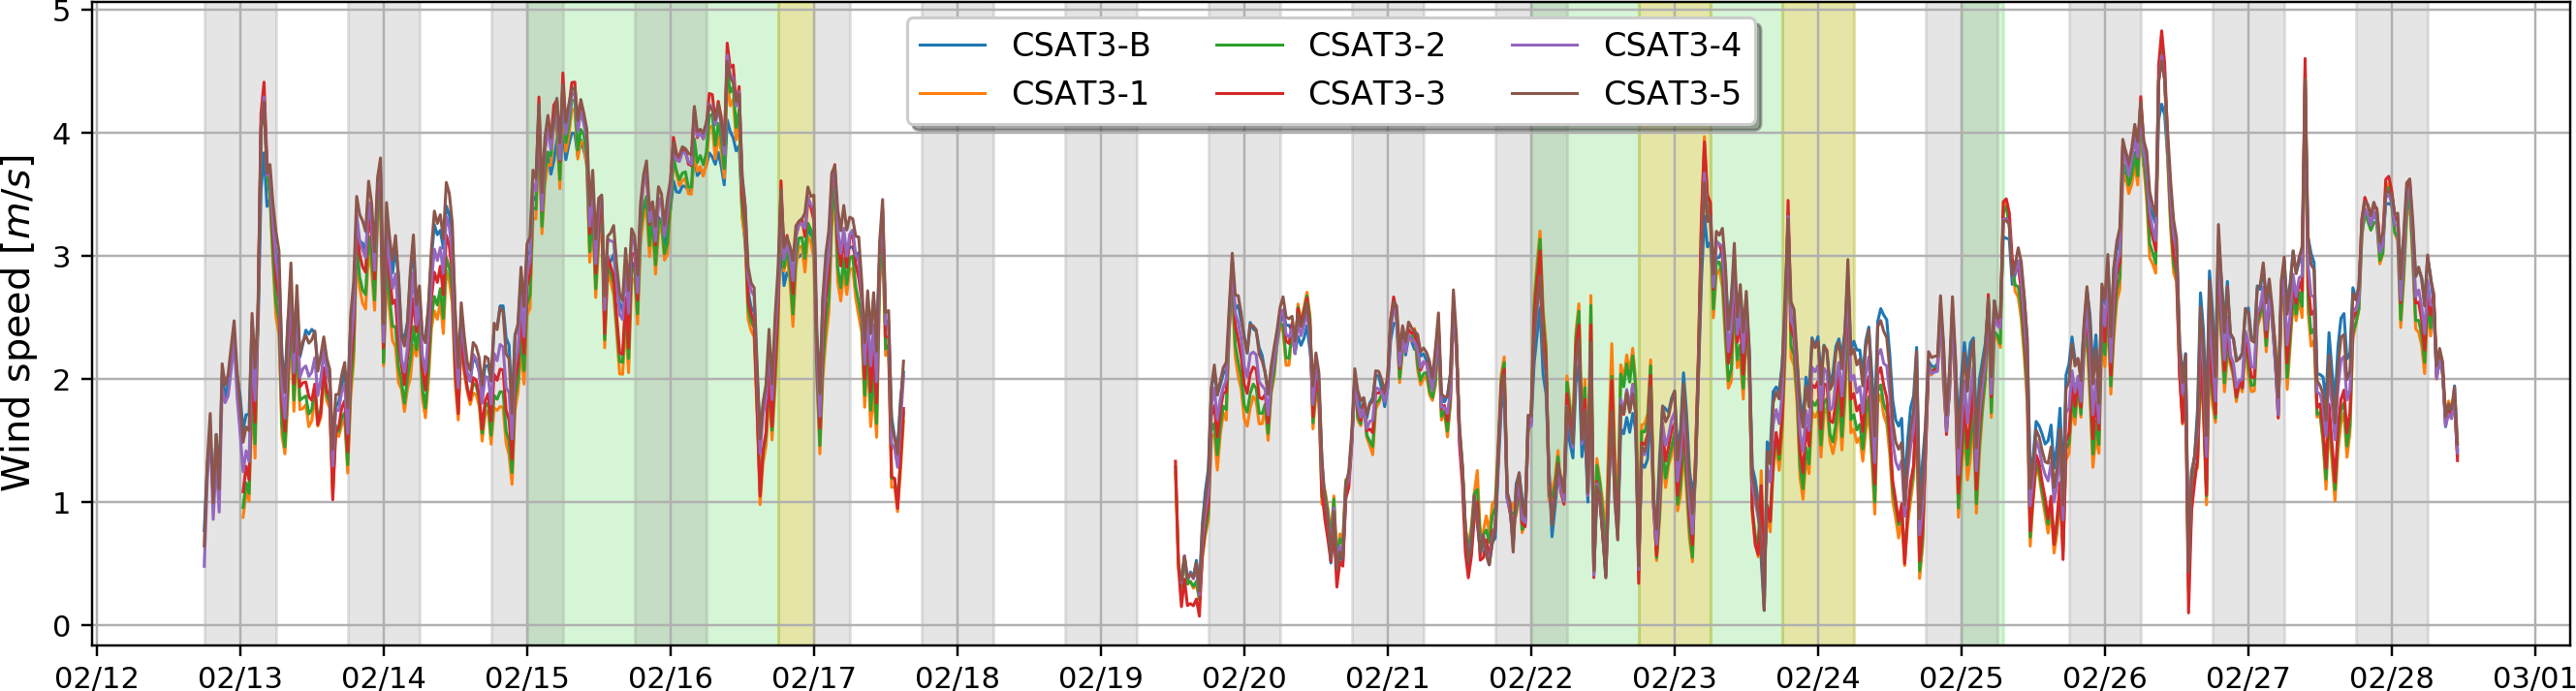
\includegraphics[width=1\textwidth]{fig/chapter_4/wind_speed_csat.png} \\
   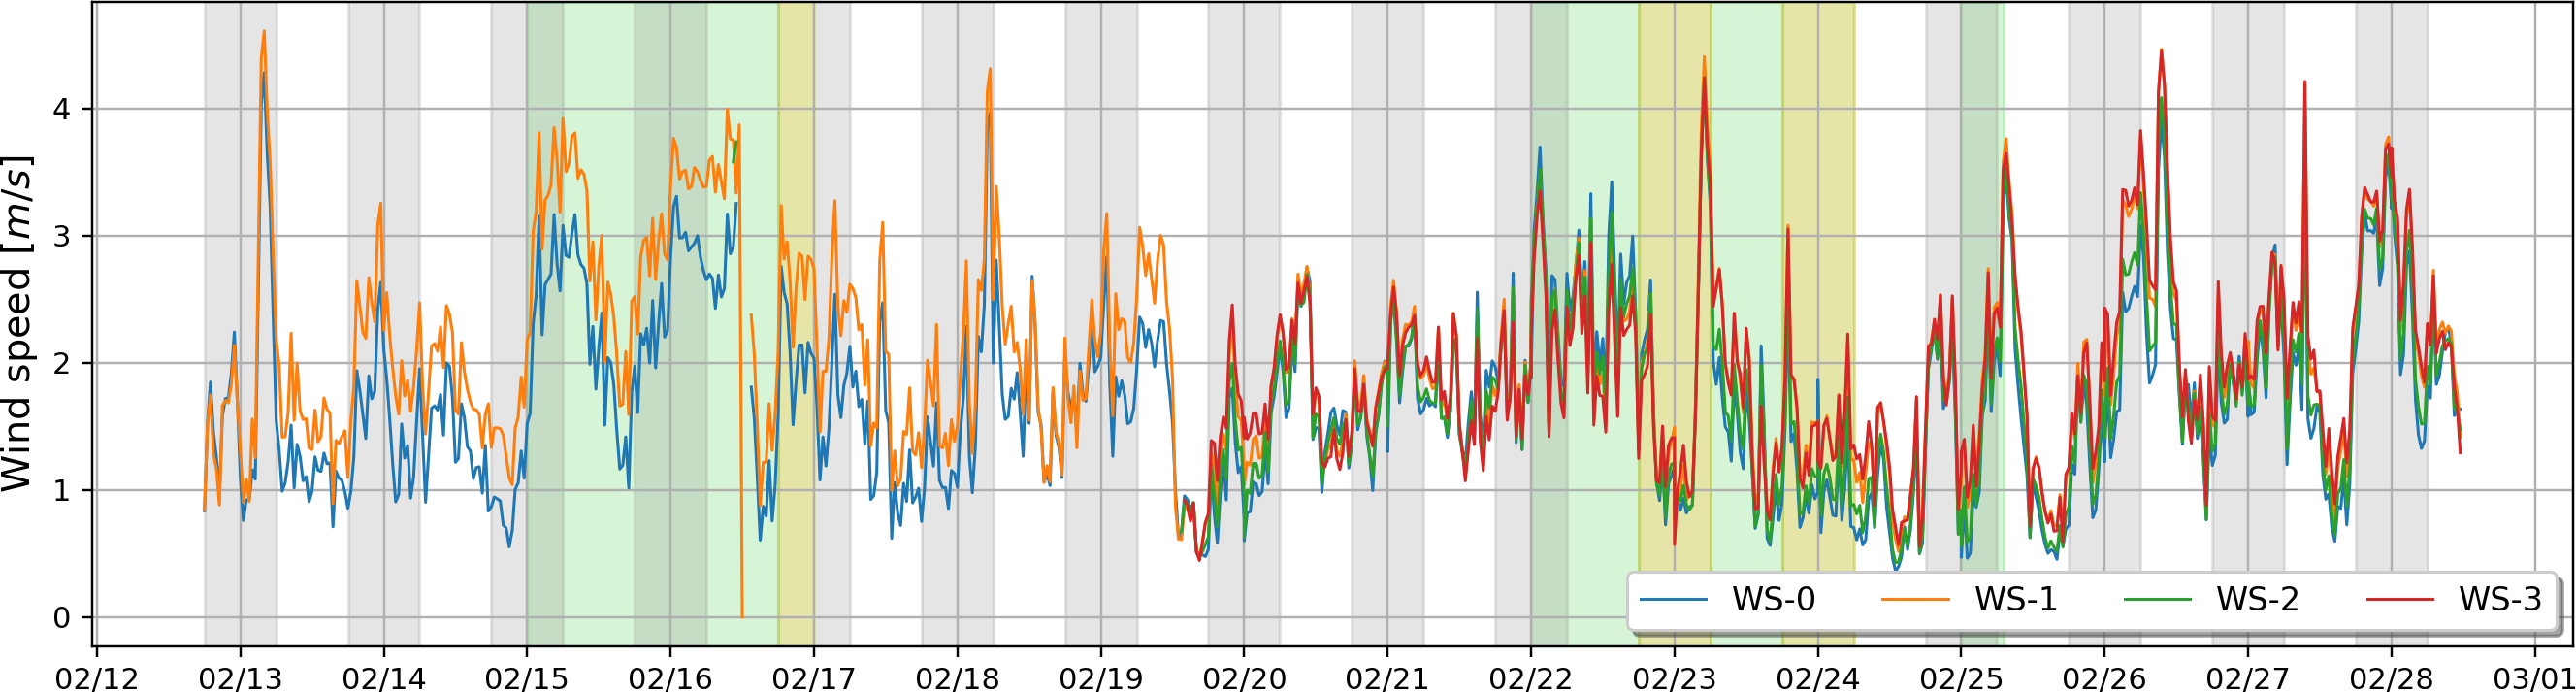
\includegraphics[width=1\textwidth]{fig/chapter_4/wind_speed_ws.png}
   }
  \caption{}
  \label{fig:windspeed_series}
\end{sidewaysfigure}